% !TEX TS-program = pdflatex
% !TEX encoding = UTF-8 Unicode

% This is a simple template for a LaTeX document using the "article" class.
% See "book", "report", "letter" for other types of document.

\documentclass[11pt]{article} % use larger type; default would be 10pt

\usepackage[utf8]{inputenc} % set input encoding (not needed with XeLaTeX)

%%% Examples of Article customizations
% These packages are optional, depending whether you want the features they provide.
% See the LaTeX Companion or other references for full information.

%%% PAGE DIMENSIONS
\usepackage{geometry} % to change the page dimensions
\geometry{a4paper} % or letterpaper (US) or a5paper or....
% \geometry{margin=2in} % for example, change the margins to 2 inches all round
% \geometry{landscape} % set up the page for landscape
%   read geometry.pdf for detailed page layout information

\usepackage{graphicx} % support the \includegraphics command and options

% \usepackage[parfill]{parskip} % Activate to begin paragraphs with an empty line rather than an indent

%%% PACKAGES
\usepackage{booktabs} % for much better looking tables
\usepackage{array} % for better arrays (eg matrices) in maths
\usepackage{paralist} % very flexible & customisable lists (eg. enumerate/itemize, etc.)
\usepackage{verbatim} % adds environment for commenting out blocks of text & for better verbatim
\usepackage{subfig} % make it possible to include more than one captioned figure/table in a single float
% These packages are all incorporated in the memoir class to one degree or another...

%%% HEADERS & FOOTERS
\usepackage{fancyhdr} % This should be set AFTER setting up the page geometry
\pagestyle{fancy} % options: empty , plain , fancy
\renewcommand{\headrulewidth}{0pt} % customise the layout...
\lhead{}\chead{}\rhead{}
\lfoot{}\cfoot{\thepage}\rfoot{}

%%% SECTION TITLE APPEARANCE
\usepackage{sectsty}
\allsectionsfont{\sffamily\mdseries\upshape} % (See the fntguide.pdf for font help)
% (This matches ConTeXt defaults)

%%% ToC (table of contents) APPEARANCE
\usepackage[nottoc,notlof,notlot]{tocbibind} % Put the bibliography in the ToC
\usepackage[titles,subfigure]{tocloft} % Alter the style of the Table of Contents
\renewcommand{\cftsecfont}{\rmfamily\mdseries\upshape}
\renewcommand{\cftsecpagefont}{\rmfamily\mdseries\upshape} % No bold!

%%% END Article customizations

%%% The "real" document content comes below...

\title{CS12420 Assignment 2, individual project}
\author{Jacob Smith, jas32}
%\date{} % Activate to display a given date or no date (if empty),
         % otherwise the current date is printed 

\begin{document}
\maketitle

\section{Changes to given design}
It is because of a desire to allow for Inventory files to be cold-swapped that all of the associations in the data package are compositions and not aggregations. This does mean that the only way to compare objects (for filtering for example) must be done in depth, rather than by a shallow method. But this does allow for an inventory to be modified to increase the price of an item - without the change being applied retroactively to the log. It is hoped that this is sufficient to justify the repetition of data.

\subsection{uk.ac.aber.dcs.cs12420.aberpizza.data.Till}
It was decided that the Till is serialised day-by-day. This requires the solution to be able to open arbitrary till logs (using \emph{load(File):Till} to open logs for previous days. In order to format the Date object (in miliseconds since 1st Jan 1970) into a human-recogniseable date (of the form YYYY-MM-DD) for use in the logs' filenames, when saved, \emph{niceDate(Date):String} is used. This makes \emph{save()} easier to read. \emph{setOrders(LinkedList)} is needed to allow XMLEncoder to serialise the orders attribute - as it requires setters and getters for all persistent attributes.

\subsection{uk.ac.aber.dcs.cs12420.aberpizza.data.Order}
In order to allow discounts to be changed, while preserving the integrity of existing Till log files the discounts applied to a given order are copied into \emph{appliedDiscounts}. In order to distinguish between an order that is under construction (with references to 'current' \emph{Item} objects) and one which is historical (from a log), the \emph{finalised:boolean} field is used. The \emph{items} private field in the given specification has been replaced with the \emph{orderTable:Map}, to better describe what it is, however the interface has been preserved. There was some confusion as to what the difference between \emph{addItem(Item,int)} and \emph{updateItemQuantity(Item,int)} was so a decision was made, \emph{addItem} 'sets' an item to a given quantity, while \emph{updateItemQuantity} increases or decrements it by the given value. The latter is implemented as a sugar for the former, reducing the amount of code to be maintained. Finally setters and getters were added to allow persistence through XMLEncoder.

\subsection{uk.ac.aber.dcs.cs12420.aberpizza.data.Item}
To allow for Pizzas to come in three sizes, and allow for other items to have multiple sizes (drinks for example), \emph{size:double} was added to the Item interface. Ignoring this attribute has no detrimental effect provided description remains unique - so it is safe to ignore this alteration. Using this alteration however allows for items to be grouped together by description in the GUI.

Three implementations of Item are provided, \emph{PizzaItem}, \emph{DrinkItem} and \emph{SideItem}; these represent a pizza, a drink, and a side-order respectively.

\subsection{uk.ac.aber.dcs.cs12420.aberpizza.data.Discount}
As mentioned previously, because of the need to make Till logs independent of reasonable changes to source code an Order contains a collection of cloned Discount objects with a \emph{BigDecimal} persisting the amount of discount that was applied at the time the sale was made. This means that even if \emph{BOGOFDiscount} was changed to recognise 'Buy 3 Get 2 Free' patterns (instead of 'Buy 1 Get 1') the change would not apply retroactively.

\emph{BOGOFDiscount} is the only implementation provided as an example. Other discount types can be added by implementing \emph{match(Order):int} to match the desired pattern in the \emph{Order}. As an example, a £10 discount on orders of value greater than £40 could be implemented by returning 1 if and only if the summed price of all items were over that threshold value.

\subsection{uk.ac.aber.dcs.cs12420.aberpizza.data.Inventory}
\emph{Inventory} was added to store all of the items and discounts currently in the store. Because Till logs contain their own, separate, copies of objects there is no need to keep a historic item in the Inventory - deleting it removes it from sale.

An \emph{Inventory} populates itself from an XML file either in the JAR or a data directory. At present the JAR is the default location and it will only load from the filesystem in the event of failure. This could be changed to allow the inventory to be editable by a user. As this was not a part of the use-case the InventoryEditor in the pipeline package is only a helper script for the developer and is not robust enough for deployment.

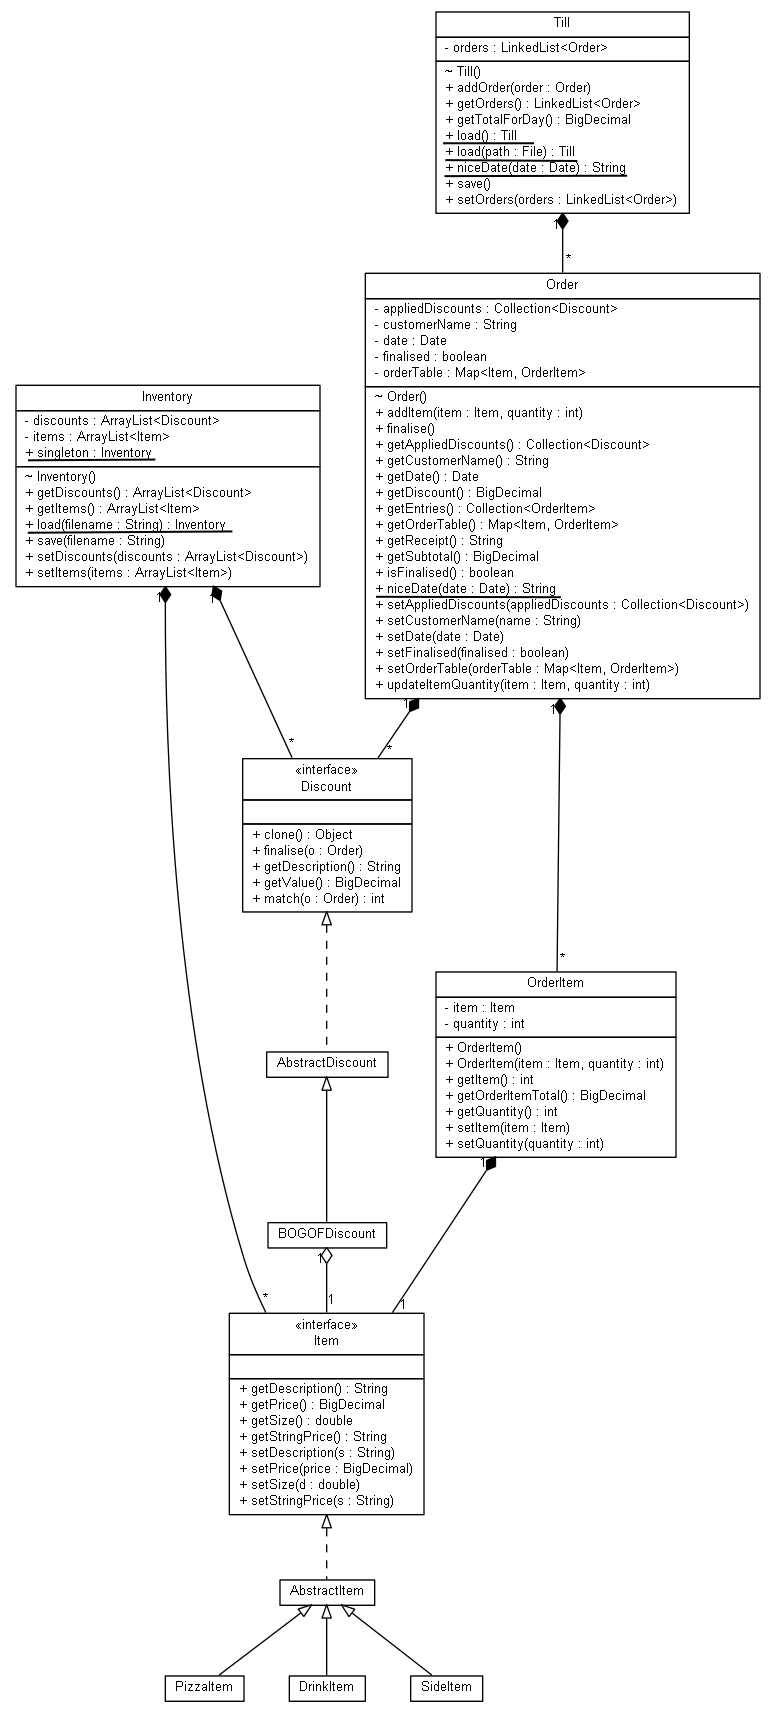
\includegraphics[scale=0.35]{classdiagram.png}

\end{document}
